\section{Příklad 2}
% Jako parametr zadejte skupinu (A-H)
\druhyZadani{F}
Úprava:

\begin{figure}[!ht]
  \centering
  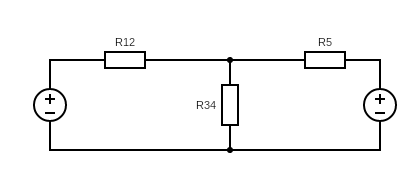
\includegraphics[width=0.6\textwidth, keepaspectratio]
  {/home/tjoslef/skola/zapisky/vut/IEL/projekt/priklad2.png}
  \caption{Další úprava}
\end{figure}


\[
    R_i = \frac{R_{12} \times R_5}{R_{12} + R_5}
\]
\[
    R_i = \frac{950 \times 80}{950 + 80} \quad \Rightarrow \quad R_i = 73.786
\]
\[
    I_x = \frac{U_2 - U_1}{R_{12} + R_5}
\]
\[
    I_x = \frac{180 - 130}{950 + 80} \quad \Rightarrow \quad I_x = 0.049
\]
\[
    U_i = U_1 + R_i \times I_x
\]
\[
    U_i = 130 + 950 \times 0.049
\]
\[
    I_{R34} = \frac{U_i}{R_i + R_{34}}
\]
\[
    \frac{176.55}{73.786 + 150} \quad \Rightarrow \quad I_{R34} = 0.789
\]
\[
    U_{R34} = 0.789 \times 150 \quad \Rightarrow \quad U_{R34} = 118.35 \, \text{V}
\]
\[
    U_{R4} = 118.35 \, \text{V}
\]
\[
    I_{R4} = \frac{118.35}{650} \quad \Rightarrow \quad I_{R3} = 0.1821 \, \text{A}
\]

